\documentclass{llncs}
\usepackage{amsmath,amssymb,calc,ifthen}
\usepackage{float}
%\usepackage{cancel}
\usepackage[table,usenames,dvipsnames]{xcolor} % for coloured cells in tables
\usepackage{tikz}
% Allows us to click on links and references!
\usepackage{hyperref}
\usepackage{url}
\hypersetup{
colorlinks,
citecolor=black,
filecolor=black,
linkcolor=black,
urlcolor=black
}
% Nice package for plotting graphs
% See excellent guide:
% http://www.tug.org/TUGboat/tb31-1/tb97wright-pgfplots.pdf
\usetikzlibrary{plotmarks,shapes}
\usepackage{amsmath,graphicx}
\usepackage{epstopdf}
%\usepackage{caption}
\usepackage{subcaption}
\usepackage{graphicx}
% highlight - useful for TODOs and similar
\usepackage{color}
\newcommand{\hilight}[1]{\colorbox{yellow}{#1}}
\newcommand\ci{\perp\!\!\!\perp} % perpendicular sign
\newcommand*\rfrac[2]{{}^{#1}\!/_{#2}} % diagonal fraction
\newcommand\SLASH{\char`\\}
\usepackage{listings}
% margin size
\usepackage{pdfpages}
\usepackage{enumitem} % for nested enumerate numbers 1 1.1 1.1.1
% \usepackage{breqn}
% \usepackage[linesnumbered]{algorithm2e}
% \usepackage{algorithmicx,algpseudocode}
% \usepackage{wrapfig} % for allowing text wrapped around the algorithm
% \newcommand\mycommfont[1]{\footnotesize\ttfamily\textcolor{blue}{#1}}
% \SetCommentSty{mycommfont}

% \usepackage{titlesec}
% \titlespacing*{\section}
% {0pt}{5.5ex plus 1ex minus .2ex}{4.3ex plus .2ex}

\usepackage[linesnumbered]{algorithm2e}
\newcommand\mycommfont[1]{\footnotesize\ttfamily\textcolor{blue}{#1}}
\SetCommentSty{mycommfont}



\DeclareMathOperator*{\argmin}{arg\,min}
\DeclareMathOperator*{\argmax}{arg\,max}

\begin{document}

\definecolor{blue3}{HTML}{86B7FC} % med blue
\definecolor{blue1}{HTML}{B5F1FF} % light blue
\definecolor{blue2}{HTML}{E0F9FF} % very light blue

\title{Disease Knowledge Transfer across Neurodegenerative Diseases}
%
\titlerunning{Disease Knowledge Transfer across Alzheimer's Variants}  % abbreviated title (for running head)
%                                     also used for the TOC unless
%                                     \toctitle is used
%

% * <mrazvan22@gmail.com> 2018-03-02T16:41:47.321Z:
% 
% Author list: Me, Marco (writing+model code), Pere (helped with validation), Alex (writing+tadpole), Neil (tadpole),  Arman, Keir (DTI data), Seb, Danny
% 
% ^ <mrazvan22@gmail.com> 2018-03-02T16:55:06.003Z.

\author{*******************************************}

\institute{***************************************}


\maketitle              % typeset the title of the contribution


\newcommand{\expFld}{../resfiles/tad-drcTiny_JMD}
\newcommand{\jmdFld}{..}

\begin{abstract}
We introduce Disease Knowledge Transfer (DKT), a novel technique for transferring biomarker information between related neurodegenerative diseases. DKT infers robust multimodal biomarker trajectories in rare neurodegenerative diseases even when only limited, unimodal data is available, by transferring information from larger multimodal datasets from common neurodegenerative diseases. DKT is a joint-disease generative model of biomarker progressions, which exploits biomarker relationships that are shared across diseases. As opposed to current deep learning approaches, DKT is interpretable, which allows us to understand underlying disease mechanisms, and can also predict the future evolution of subjects instead of solving simpler control vs diseased classification tasks. Here we demonstrate DKT on Alzheimer's disease (AD) variants and its ability to predict trajectories for multimodal biomarkers in Posterior Cortical Atrophy (PCA), in lack of such data from PCA subjects. For this we train DKT on a combined dataset containing subjects with two distinct diseases and sizes of data available: 1) a larger, multimodal typical AD dataset (tAD) from the TADPOLE Challenge, and 2) a smaller unimodal Posterior Cortical Atrophy (PCA) dataset from our own centre, for which only a limited number of Magnetic Resonance Imaging (MRI) scans are available. We first show that the estimated multimodal trajectories in PCA are plausible as they agree with previous literature. We further validate DKT in two situations: (1) on synthetic data, showing that it can accurately estimate the ground truth parameters and (2) on 20 DTI scans from controls and PCA patients, showing that it has favourable performance compared to standard approaches. While we demonstrated DKT on Alzheimer's variants, we note DKT is generalisable to other forms of related neurodegenerative diseases. Our code is available online: \url{https://www.dropbox.com/s/yotur0ohvgwc8om/dkt.zip?dl=0} (anonymised link).

\keywords{Disease Progression Model, Transfer Learning, Manifold Learning, Alzheimer's Disease, Posterior Cortical Atrophy}
\end{abstract}

\section{Introduction}


The estimation of accurate biomarker signatures in Alzheimer's disease (AD) and related neurodegenerative diseases is crucial for understanding underlying disease mechanisms, predicting subjects' progressions, and enrichment in clinical trials. Recently, several data-driven disease progression models were proposed to reconstruct long term biomarker signatures from collections of short term individual measurements \cite{lorenzi2017disease,oxtoby2018}. When applied to large datasets of typical AD, disease progression models have shown important benefits in understanding the earliest events in the AD cascade \cite{iturria2016early}, quantifying biomarkers' heterogeneity \cite{young2018uncovering}, helped discover novel genes involved in AD \cite{scelsi2018genetic} and they showed improved predictions over standard approaches \cite{oxtoby2018}. However, by necessity these models require large datasets -- in addition they must be both multimodal and longitudinal. Such data is not available in rare neurodegenerative diseases. In particular, most datasets for rare neurodegenerative diseases come from local clinical centres, are unimodal (e.g. MRI only) and limited both cross-sectionally and longitudinally -- this makes the application of disease progression models extremely difficult.  Moreover, such a model estimated from common diseases such as typical AD may not generalise to specific variants. For example, in Posterior Cortical Atrophy (PCA) -- a neurodegenerative syndrome causing visual disruption -- posterior regions such as the occipital lobe and superior parietal regions are affected early, instead of the hippocampus and temporal regions that are affected early in typical AD. 

The problem of limited data in medical imaging has so far been addressed through transfer learning methods. These techniques successfully used transfer learning techniques to improve the accuracy of AD diagnosis \cite{hon2017towards,cheng2017multi} or prediction of MCI conversion \cite{cheng2015domain}, but have two key limitations. First, they use deep learning or other machine learning methods, which are not interpretable and don't allow us to understand underlying disease mechanisms that are either specific to rare diseases, or shared across related diseases. Secondly, these models cannot be used to forecast the future evolution of subjects at risk of disease, which is important for selecting the right subjects in clinical trials. 

We propose Disease Knowledge Transfer (DKT), a generative joint model that estimates continuous multimodal biomarker progressions for multiple neurodegenerative diseases simultaneously -- including rare neurodegenerative diseases -- and which inherently performs transfer learning between the modelled phenotypes. This is achieved by exploiting biomarker relationships that are shared across diseases, whilst accounting for differences in the spatial distribution of brain pathology. DKT is interpretable, which allows us to understand underlying disease mechanisms, and can also predict the future evolution of subjects at risk of diseases. We apply DKT on Alzheimer's variants and demonstrate its ability to predict non-MRI trajectories for patients with Posterior Cortical Atrophy, in lack of such data. This is done by fitting DKT to two datasets simultaneously: (1) the TADPOLE Challenge \cite{marinescu2018tadpole} dataset containing subjects from the Alzheimer's Disease Neuroimaging Initiative (ADNI) with MRI, FDG-PET, DTI, AV45 and AV1451 scans and (2) MRI scans from patients with Posterior Cortical Atrophy from the Dementia Research Centre (DRC), UK. We first show that the estimated non-MRI trajectories for PCA subjects are plausible as they agree with previous literature findings. We further validate DKT on simulated data from two synthetic diseases with known ground truth, and a set of 20 DTI scans from controls and PCA patients, showing it yields favourable performance compared to standard approaches. Code for DKT is available online: \url{https://www.dropbox.com/s/yotur0ohvgwc8om/dkt.zip?dl=0} (anonymised link).

\begin{figure}[h]
 \centering
 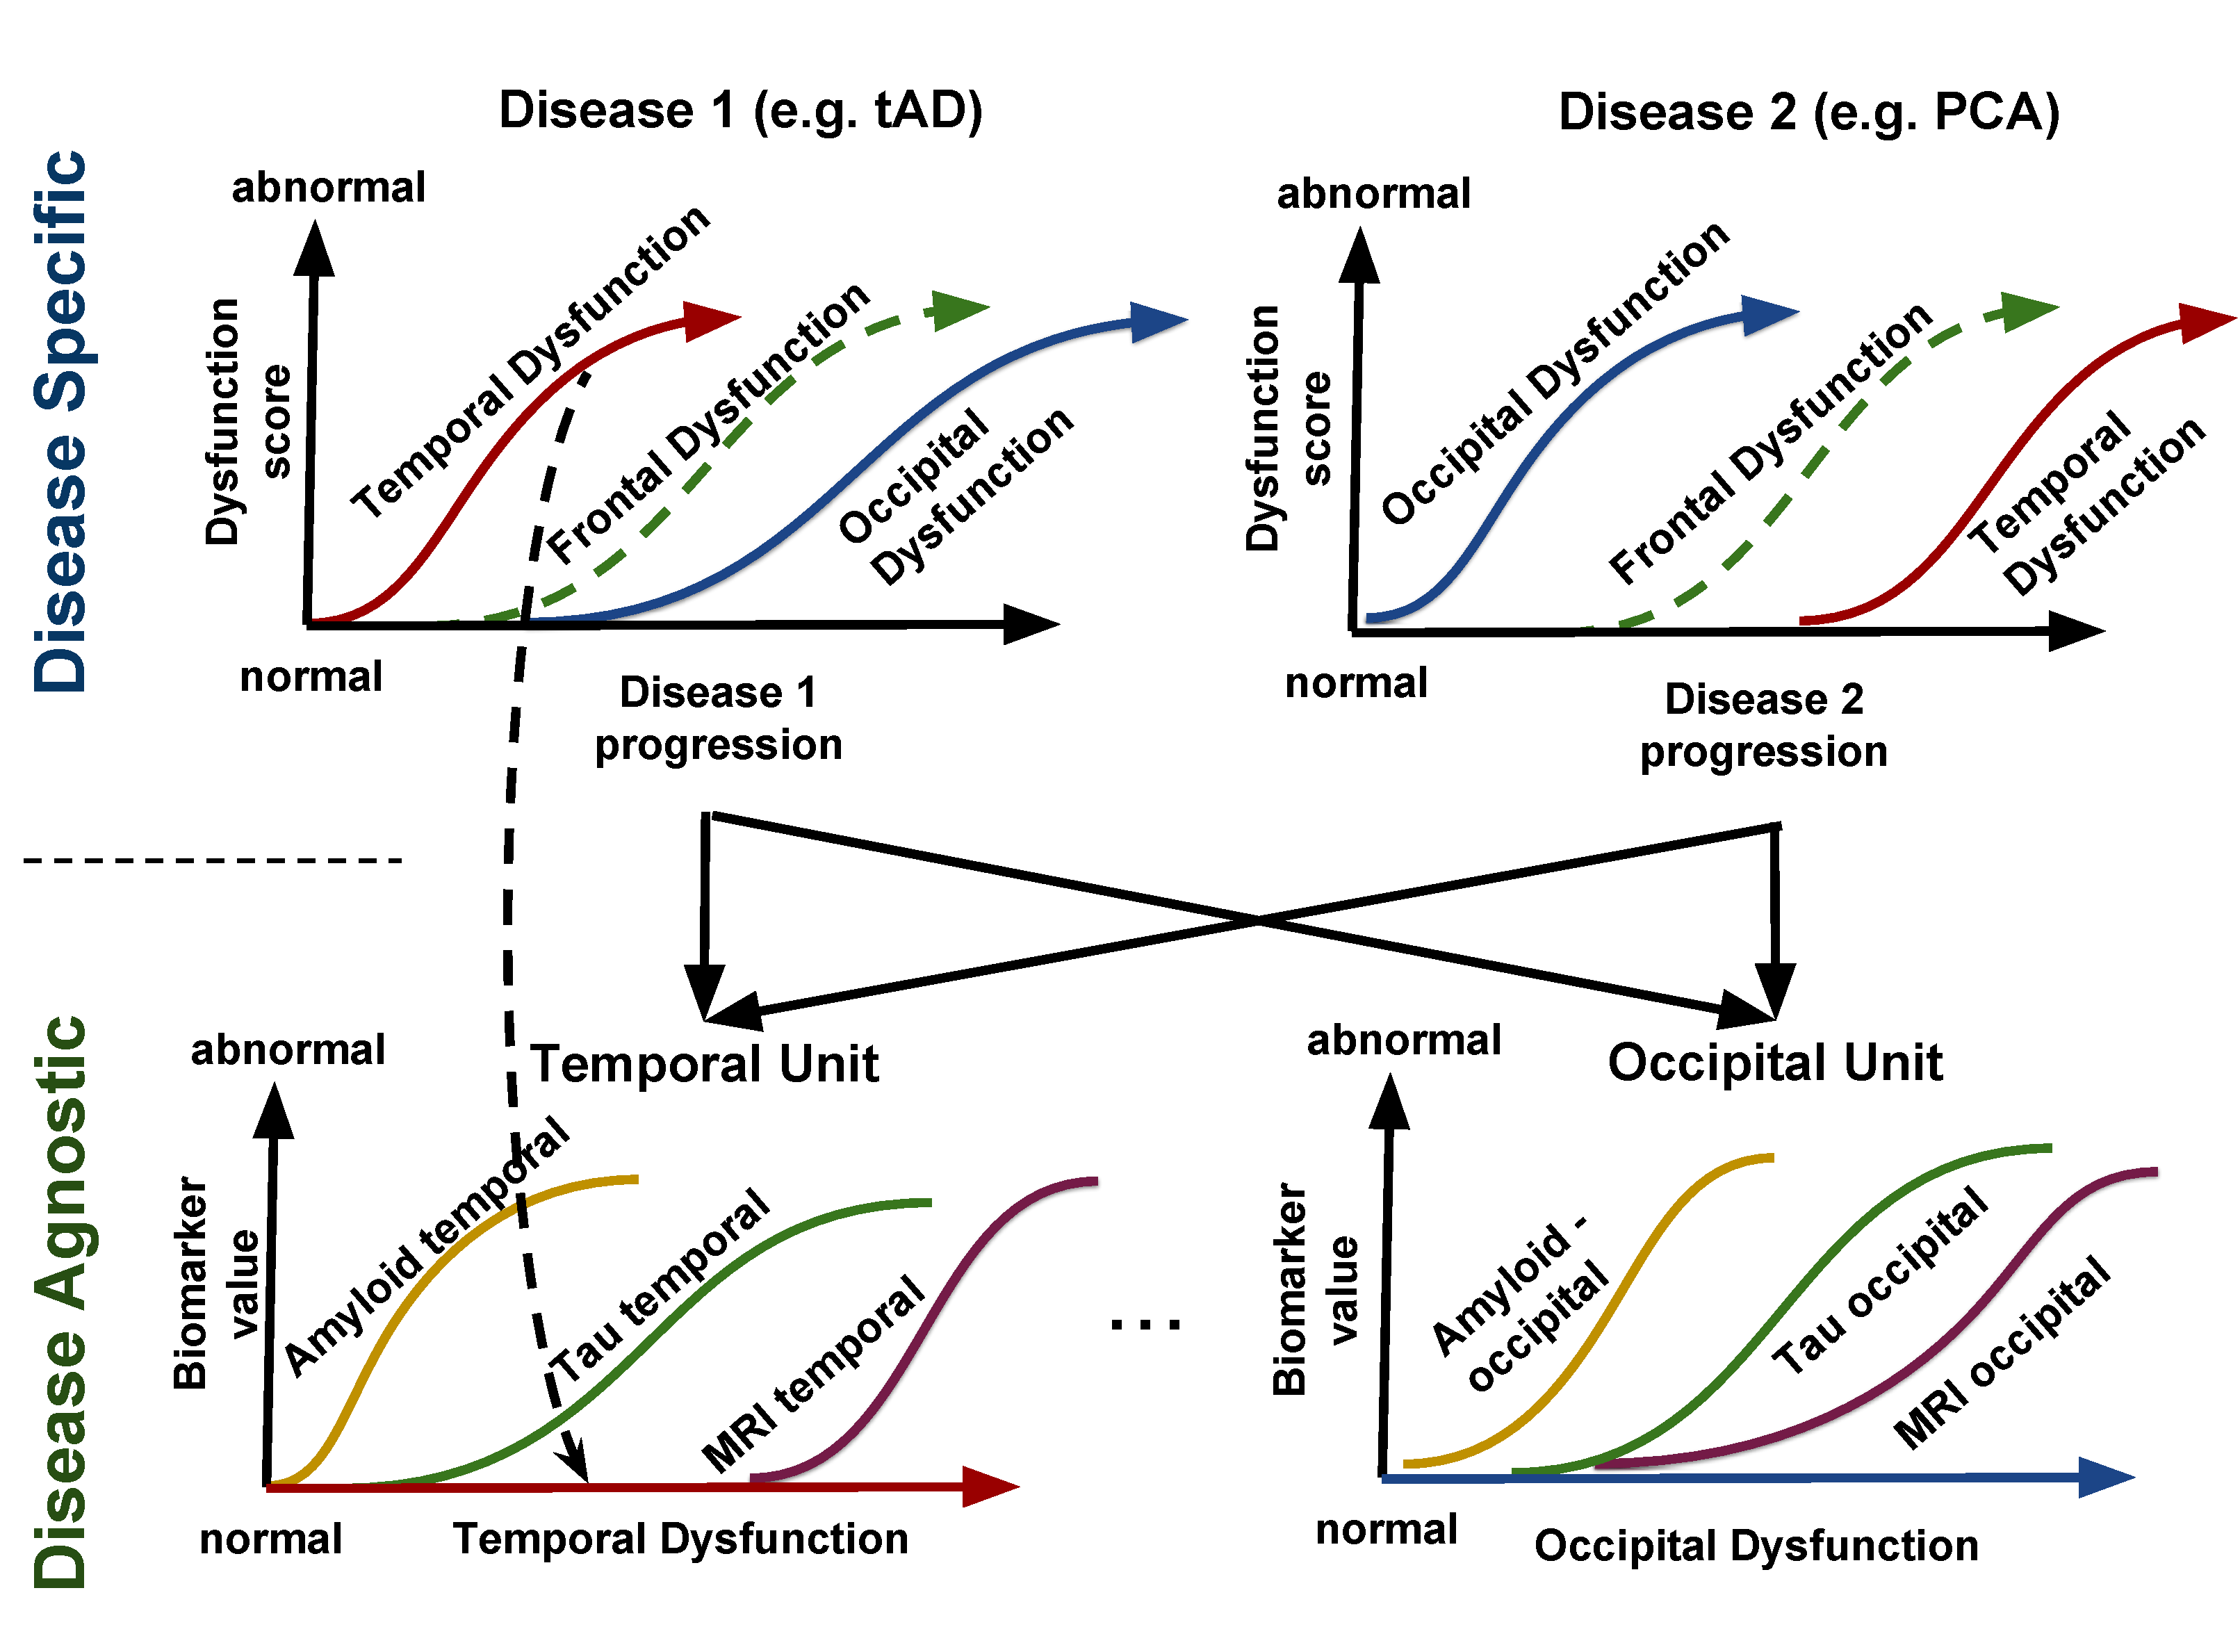
\includegraphics[width=0.8\textwidth,trim=0 0 0 0,clip]{figures/disease_knowledge_transfer.pdf}
 \caption{Diagram of the proposed DKT framework. We assume that each disease can be modelled as the evolution of abstract dysfunctionality scores (Y-axis, top row), each one related to different brain regions. Each region-specific dysfunctionality score then further models (X-axis, bottom row) the progression of several modality-specific biomarkers within that same region. For instance, the temporal dysfunction, modelled as a biomarker in the disease specific model (top row), is the X-axis in the disease agnostic model (temporal unit, bottom row), which aggregates together abnormality from amyloid, tau and MR imaging within the temporal lobe. The biomarker correlations within the bottom units are assumed to be disease agnostic and shared across all diseases modelled. Disease knowledge transfer can then be achieved via the disease-agnostic units.}
 \label{fig:diagram}
\end{figure}

\section{Method}

\newcommand{\lp}{\lambda_{d_i}^{\psi(k)}}
\newcommand{\lpuu}{\lambda_{d_i}^{\psi(k),(u)}}
\newcommand{\lpum}{\lambda_{d_i}^{\psi(k),(u-1)}}

Fig. \ref{fig:diagram} shows the overall diagram of our proposed framework for joint modelling of diseases. We assume that the progression of each disease (X-axis, top row) can be modelled as a unique evolution of abstract dysfunctionality scores, each one related to different brain regions (top row). Each dysfunctionality score is an abstract measure of pathology within that brain region, derived from several multimodal biomarkers (e.g. amyloid, tau, MRI). 

Each dysfunctionality score is modelled as the progression of several biomarkers within that same region, but acquired using different types of modalities (Fig. \ref{fig:diagram} bottom row). Each group of biomarkers in the bottom row will be called an \emph{agnostic unit}, because the biomarker dynamics are shared across all diseases modelled (i.e. disease agnostic).

The assumption that the dynamics of some biomarkers are agnostic, or shared across diseases, is key to DKT. There are several reasons why we can make this assumption: first of all, neurodegenerative diseases are known

We choose to model the correlations within each unit using the disease progression model (DPM) by Jedynak et al. 2012, but any other DPM can also be used. The DPM allows us to reconstruct unit-specific dysfunction progression manifolds (bottom row, X axis), which can be used for staging subjects. Finally, we use the same model to express the progression within each disease (Figure 1, top) in terms of the dysfunction scores estimated within each agnostic unit. More precisely, the X-axis dysfunction scores from the agnostic units become Y-axis measurements in the disease specific models.

\subsection{Mathematical formulation}

The DKT framework has a generic mathematical formulation which uses several disease progression models as building blocks. We will first describe the generic framework, and in the following section we will present our chosen implementation of the building blocks. We assume a set of given biomarkers measurements $Y = [y_{ijk} | (i,j,k) \in \Omega]$ for subject $i$ at visit $j$ in biomarker $k$, where $\Omega$ is defined as the set of available biomarker measurements, since subjects can have missing biomarkers at various visits. We assume that each subject $i$ at each visit $j$ has an underlying disease stage $s_{ij} = \beta_i + m_{ij}$, where $m_{ij}$ represents the months since baseline visit for subject $i$ at visit $j$ and $\beta_i$ represents the time shift of subject $i$. We further denote by $\theta_k$ the parameters used to represent the trajectory for biomarker $k \in K$ within its agnostic unit $\psi(k)$, where $\psi$: \{1, ..., K\} $ \rightarrow \Lambda$ maps each biomarker $k$ to a unique agnostic unit $l \in \Lambda$, where $\Lambda$ is the set of agnostic units. Moreover, we denote by $\lambda_d^l$ the parameters for the trajectory of the dysfunction score corresponding to agnostic unit $l \in \Lambda$ in the space of disease $d$. These definitions allow us to formulate the likelihood for a single measurement $y_{ijk}$ as follows:

\begin{equation}
 p(y_{ijk}|\theta_k, \lp, \beta_i, \epsilon_k) = N(y_{ijk}| g(f(\beta_i + m_{ij}; \lp; \theta_k), \epsilon_k)
\end{equation}
where $g(\ .\ ; \theta_k)$ represents the trajectory of biomarker $k$ within agnostic unit $\psi(k)$ and $f(\ .\ ; \lambda_{d_i}^{\psi(k)})$ represents the trajectory of the agnostic unit $\psi(k)$ within the space of disease $d_i$. To be precise, $d_i \in \mathbb{D}$ represents the index of the disease space where subject $i$ belongs, where $\mathbb{D}$ is the set of all diseases modelled. For example, MCI and tAD subjects from ADNI as well as tAD subjects from the DRC cohort can all be assigned $d_i=1$, while PCA subjects from our own centre can be assigned $d_i=2$. Healthy controls can be assigned to either disease space, although a more precise assignment would take molecular biomarkers into account. Variable $\epsilon_k$ denotes the variance of measurements for biomarker $k$. 

We extend the above model to multiple subjects, visits and biomarkers to get the full model likelihood:
\begin{equation}
 p(\boldsymbol{y}|\theta, \lambda, \beta , \epsilon) = \\ \prod_{(i,j,k) \in \Omega} p(y_{ijk}|\theta_k, \lp, \beta_i) 
\end{equation}

where $\boldsymbol{y} = [y_{ijk} | \forall (i,j,k) \in \Omega ]$ is the vector of all biomarker measurements, while $\boldsymbol{\theta} = [\theta_1, ..., \theta_K]$ represents the stacked parameters for the trajectories of biomarkers in agnostic units, $\boldsymbol{\lambda} = [\lambda_d^{l}|l \in \Lambda, d \in \mathbb{D}]$ are the parameters of the dysfunctionality trajectories within the disease models, $\boldsymbol{\beta} =[\beta_1, ..., \beta_N]$ are the subject-specific time shifts and $\boldsymbol{\epsilon} = [\epsilon_k | k \in K]$  estimates biomarker measurement noise. Here we assumed independence across different subjects, but the biomarker measurements and visits are linked through the latent time-shift $\beta_i$ for each subject. The parameters of the model that need to be estimated are $[\boldsymbol{\theta}, \boldsymbol{\lambda}, \boldsymbol{\beta}, \boldsymbol{\epsilon}]$.

\subsection{Modelling Biomarker Trajectories}
\label{sec:dktBiomkTraj}

So far we defined the DKT framework using generic models $g(\ .\ ; \theta_k)$ and $f(\ .\ ; \lp)$ for the biomarker trajectories within the agnostic units and the disease models. Now we choose to implement the $f$ and $g$ models as parametric sigmoidal curves, to enable a robust optimisation and because these models account for the floor and ceiling effects normally observed in AD biomarkers \cite{sabuncu2011dynamics}. The sigmoidal model for $f$ is defined as:

\begin{equation}
 f(s;\theta_k) = \frac{a_k}{1+exp(-b_k(s-c_k))} + d_k
\end{equation}

where $s$ is the disease progression score of a subject and $\theta_k = [a_k, b_k, c_k, d_k]$ are parameters controlling the shape of the trajectory for biomarker $k$: $d_k$ and $d_k + a_k$ represent the lower and upper limits of the sigmoidal function, $c_k$ represents the inflection point and $a_k b_k/4$ represents the slope at the inflection point. A similar model is used also for $g$.


\subsection{Parameter Estimation}

\newcommand{\uu}{^{(u)}}
\newcommand{\um}{^{(u-1)}}

We estimate the model parameters using a two-stage approach. In the first stage, we perform belief propagation within each agnostic unit and then within each disease model. Each agnostic unit and disease model is assumed to be an independent disease progression model that we fit by alternatively optimising the fit of biomarker trajectories and subject-specific time-shifts, using the approach described in \cite{jedynak2012computational}. At this stage we assume the existence of a latent variable $\beta_i^{\psi(k)} = f(\beta_i + m_{ij}; \lp)$ representing the dysfunctionality score of subject $i$ within the agnostic unit $\psi(k)$, which represents a time-shift within that agnostic unit.

In the second stage we jointly optimise across all agnostic units and disease models using loopy belief propagation. An overview of the algorithm is given in Figure \ref{fig:dktAlgo}. Given the initial parameters estimated from the first stage (line 1), the algorithm continuously updates the biomarker trajectories within the agnostic units (lines 4-5), dysfunctionality trajectories (line 9) and subject-specific time shifts (line 13) until convergence. The cost function for all parameters is nearly identical, the main difference being the measurements $(i,j,k)$ over subjects $i$, visits $j$ and biomarkers $k$ that are selected for computing the measurement error. For estimating the trajectory of biomarker $k$ within agnostic unit $\psi(k)$, measurements are taken from $\Omega_k$ representing all measurements of biomarker $k$ from all subjects and visits. For estimating the dysfunctionality trajectories,  $\Omega_{d,l}$ represents the measurement indices from all subjects with disease $d$ (i.e. $d_i = d$) and all biomarkers $k$ that belong to agnostic unit $l$ (i.e. $\psi(k) = l$). Finally, $\Omega_i$ (line 13) represents all measurements from subject $i$, for all biomarkers and visits. 


\begin{figure}
\begin{algorithm}[H]
\tiny
 Initialise $\boldsymbol{\theta}^{(0)}$, $\boldsymbol{\lambda}^{(0)}$, $\boldsymbol{\beta}^{(0)}$\\
  \While{$\boldsymbol{\theta}$, $\boldsymbol{\lambda}$, $\boldsymbol{\beta}$ not converged}{
   \tcp*[l]{Estimate biomarker trajectories (disease agnostic)}
    \For{$k=1$ to $K$}{
      ${\theta_k\uu = \argmin_{\theta_k} \sum_{(i,j) \in \Omega_k} \left[y_{ijk} - g\left(f(\beta_i\um + m_{ij}; \lpum) ; \theta_k\right) \right]^2  - log\ p(\theta_k)}$\\
      ${\epsilon_k\uu = \frac{1}{|\Omega_k|} \sum_{(i,j) \in \Omega_k}    \left[y_{ijk} - g\left(f(\beta_i\um + m_{ij}; \lpum) ; \theta_k\uu \right) \right]^2 }$\\
    }
     \tcp*[l]{Estimate dysfunctionality trajectories (disease specific)} 
    \For{$d=1 \in \mathbb{D}$}{
      \For{$l=1 \in \Lambda$}{
        ${\lambda_{d}^{l, (u)} = \argmin_{\lambda_{d}^{l}} \sum_{(i,j,k) \in \Omega_{d,l}} \left[y_{ijk} - g\left(f(\beta_i\um + m_{ij}; \lambda_{d}^{l}) ; \theta_k\uu 
        \right) \right]^2  - log\ p(\lambda_{d}^{l})}$\\
      }
    }
    \tcp*[l]{Estimate subject-specific time shifts} 
    \For{$i=1 \in [1, \dots, S]$}{
      ${\beta_i\uu = \argmin_{\beta_i} \sum_{(j,k) \in \Omega_i} \left[y_{ijk} - g\left(f(\beta_i + m_{ij}; \lpuu) ; \theta_k\uu
      \right) \right]^2  - log\ p(\beta_i)}$\\
    }
}
\normalfont
\end{algorithm}
\caption[The algorithm for estimating the DKT parameters]{The algorithm for estimating the DKT parameters. The algorithm successively updates the biomarker trajectories within the agnostic units (disease agnostic models), dysfunctionality trajectories (disease specific) and subject-specific time shifts until convergence.}
\label{fig:dktAlgo}
\end{figure}



\subsection{Generating Synthetic Data}
\label{sec:dktMetSyn}

We first test DKT on synthetic data, in order to assess the performance when ground truth is known. We generate synthetic data from two diseases as follows:
\begin{itemize}
 \item[] \textbf{Disease model}
 \item We define two agnostic units $l_0$ and $l_1$ and 6 biomarkers $k_0-k_6$, which we allocate to agnostic units as follows: $l_0:\{k_0, k_2, k_4\}$, $l_1: \{k_1, k_3, k_5\}$. Within their units, we define the trajectory of each biomarker as a sigmoidal curves with the following $\theta_k$ parameters:
 \begin{itemize}
  \item agnostic unit $l_0$: $\theta_0 = (1,5,0.2,0)$, $\theta_2 = (1,5,0.55,0)$ and $\theta_4 = (1,5,0.9,0)$ 
  \item agnostic unit $l_1$: $\theta_1 = (1,10,0.2,0)$, $\theta_3 = (1,10,0.55,0)$ and $\theta_5 = (1,10,0.9,0)$ 
 \end{itemize}
 \item We define two synthetic diseases, "synthetic AD" ($d=0$) and "synthetic PCA" ($d=1$). For each disease $d$, each agnostic unit $l$ has a distinct dysfunctionality trajectory defined as a sigmoidal curve with parameters $\lambda_d^l$ as follows: 
 \begin{itemize}
  \item "synthetic AD" disease: $\lambda_0^0 = (1, 0.3, -4, 0)$  and $\lambda_0^1 = (1, 0.2, 6, 0)$.
  \item "synthetic PCA" disease: $\lambda_1^0 = (1, 0.3, 6, 0)$ and $\lambda_1^1 = (1, 0.2, -4, 0)$.
 \end{itemize}

 \item[] \textbf{Subject model}
 \item We generated time-shifts $\beta_i$ for 100 subjects (disease $d_0$) and 50 subjects (disease $d_1$) based on a uniform distribution with ranges $(-13, 10)$ years before/after disease onset. 
 \item Within each disease, we generated the subjects' diagnosis (controls/patients) based on an exponential likelihood model with mean -4.5 (controls)/4.5 (patients) years before/after disease onset. 
 \item For each subject and each biomarker, we generated data for four consecutive visits, each visit one year apart, using a noise standard deviation of 0.05.
\end{itemize}

These trajectory and subject parameters were chosen to mimic the TADPOLE and DRC cohorts, described below. Before fitting DKT on the synthetic dataset, we discarded the data from biomarkers $k_0$, $k_1$, $k_4$ and $k_5$ for all subjects within the synthetic PCA cohort, to simulate the lack of multimodal data in these subjects. Remaining biomarkers $k_2$ and $k_3$, for which data was still available in the synthetic PCA cohort, are assumed to be of the same modality (e.g. MRI volume) but to represent measurements from different brain regions (e.g. temporal and occipital). 


\subsection{Data acquisition and Preprocessing}

We trained DKT on ADNI data from the TADPOLE challenge (Marinescu et al., arXiv, 2018), since it contained a large number of multimodal biomarkers already pre-processed and aggregated into one table. From the TADPOLE dataset we selected a subset of 230 subjects which had at least one FDG PET, AV45, AV1451 or DTI scan. Most subjects also had MRI scans and cognitive tests. In order to model another disease, we further included 76 PCA subjects from our own centre in the training set, along with 67 tAD and 87 age-matched controls, all of which only had MRI scans.
 
For both datasets, volumetric measures for each subject have been obtained using the Freesurfer software. For FDG, AV45 and AV1451 PET, we used already extracted SUVR measures from ADNI. For DTI, we used fractional anisotropy (FA) measures from white-matter regions adjacent to each lobe. For every lobe, we averaged the biomarker values for regions of interest within each lobe and regressed out the following covariates: age, gender, total intracranial volume (TIV) and dataset (ADNI vs our own dataset). Finally, we normalised the biomarker values to lie within the [0,1] range. 

For validating DKT's performance at predicting missing biomarkers in PCA, we used a separate test set of DTI scans from our own controls and PCA subjects. As this validation set was acquired at a centre different from ADNI and on different scanners, we matched the FA mean and standard deviation of our own controls to be equal to the FA mean and standard deviation of the ADNI controls. No DTI data from PCA subjects was exposed to the algorithm at training time.

\section{Results}
\label{sec:dktRes}

\subsection{Synthetic Results}
\label{sec:dktResSyn}

Fig. \ref{fig:dktSynthTrajCompTrue} shows the true and estimated subject shifts and trajectories for each agnostic unit $l$ and biomarker $k$. In the top-left figures we show scatter plots of the true shifts (y-axis) against estimated shifts (x-axis), for the 'synthetic AD' and 'synthetic PCA' diseases. On the top-right and middle-left figures, we show the trajectories of the agnostic units within disease $d=0$ (synthetic AD) and $d=1$ (synthetic PCA). In the middle-right and bottom-left figures, we show the biomarker trajectories within units $l_0$ and $l_1$. In Figure \ref{fig:dktSynthTrajDrcSpace}, we show the corresponding trajectories of PCA patients, which as opposed to Fig. \ref{fig:dktSynthTrajCompTrue}, are plotted directly against the time-shifts, as it is normally done in a classical disease progression model. We also show the true trajectories and the data of the synthetic PCA cohort.

The results in Fig. \ref{fig:dktSynthTrajCompTrue} suggest that the DKT-estimated trajectories match closely (MAE $<$ 0.058) with the true trajectories, for both the unit-trajectories within the disease-specific models and the biomarker trajectories within the disease-agnostic models. Moreover, the subject time-shifts are very close ($R^2$ $>$ 0.98) to the true time-shifts. When plotted directly against the disease space, the estimated PCA trajectories also match the true trajectories, even when there is a complete lack of such data (Fig. \ref{fig:dktSynthTrajDrcSpace}, biomarkers 0,1,4 and 5). There are however small errors in  biomarkers 0 and 5 which are due to measurement noise (confirmed by experiments with smaller noise level -- not shown here). The equivalent trajectories estimated for the synthetic AD cohort also show very good agreement with the true trajectories (results not shown here).

% \begin{figure}
% \includegraphics[width=\textwidth]{images/dkt/plotHierData611_synth1Pen5_JMD.png}
%  \caption{(top-left) (top-left) Scatter plots of the true shifts (y-axis) against estimated shifts (x-axis), for the 'synthetic AD' (left) and 'synthetic PCA' (right) diseases. (top-right and middle-left) Trajectories of unit }
%  \label{fig:dktSynthTrajHierData}
% \end{figure}

\begin{figure}
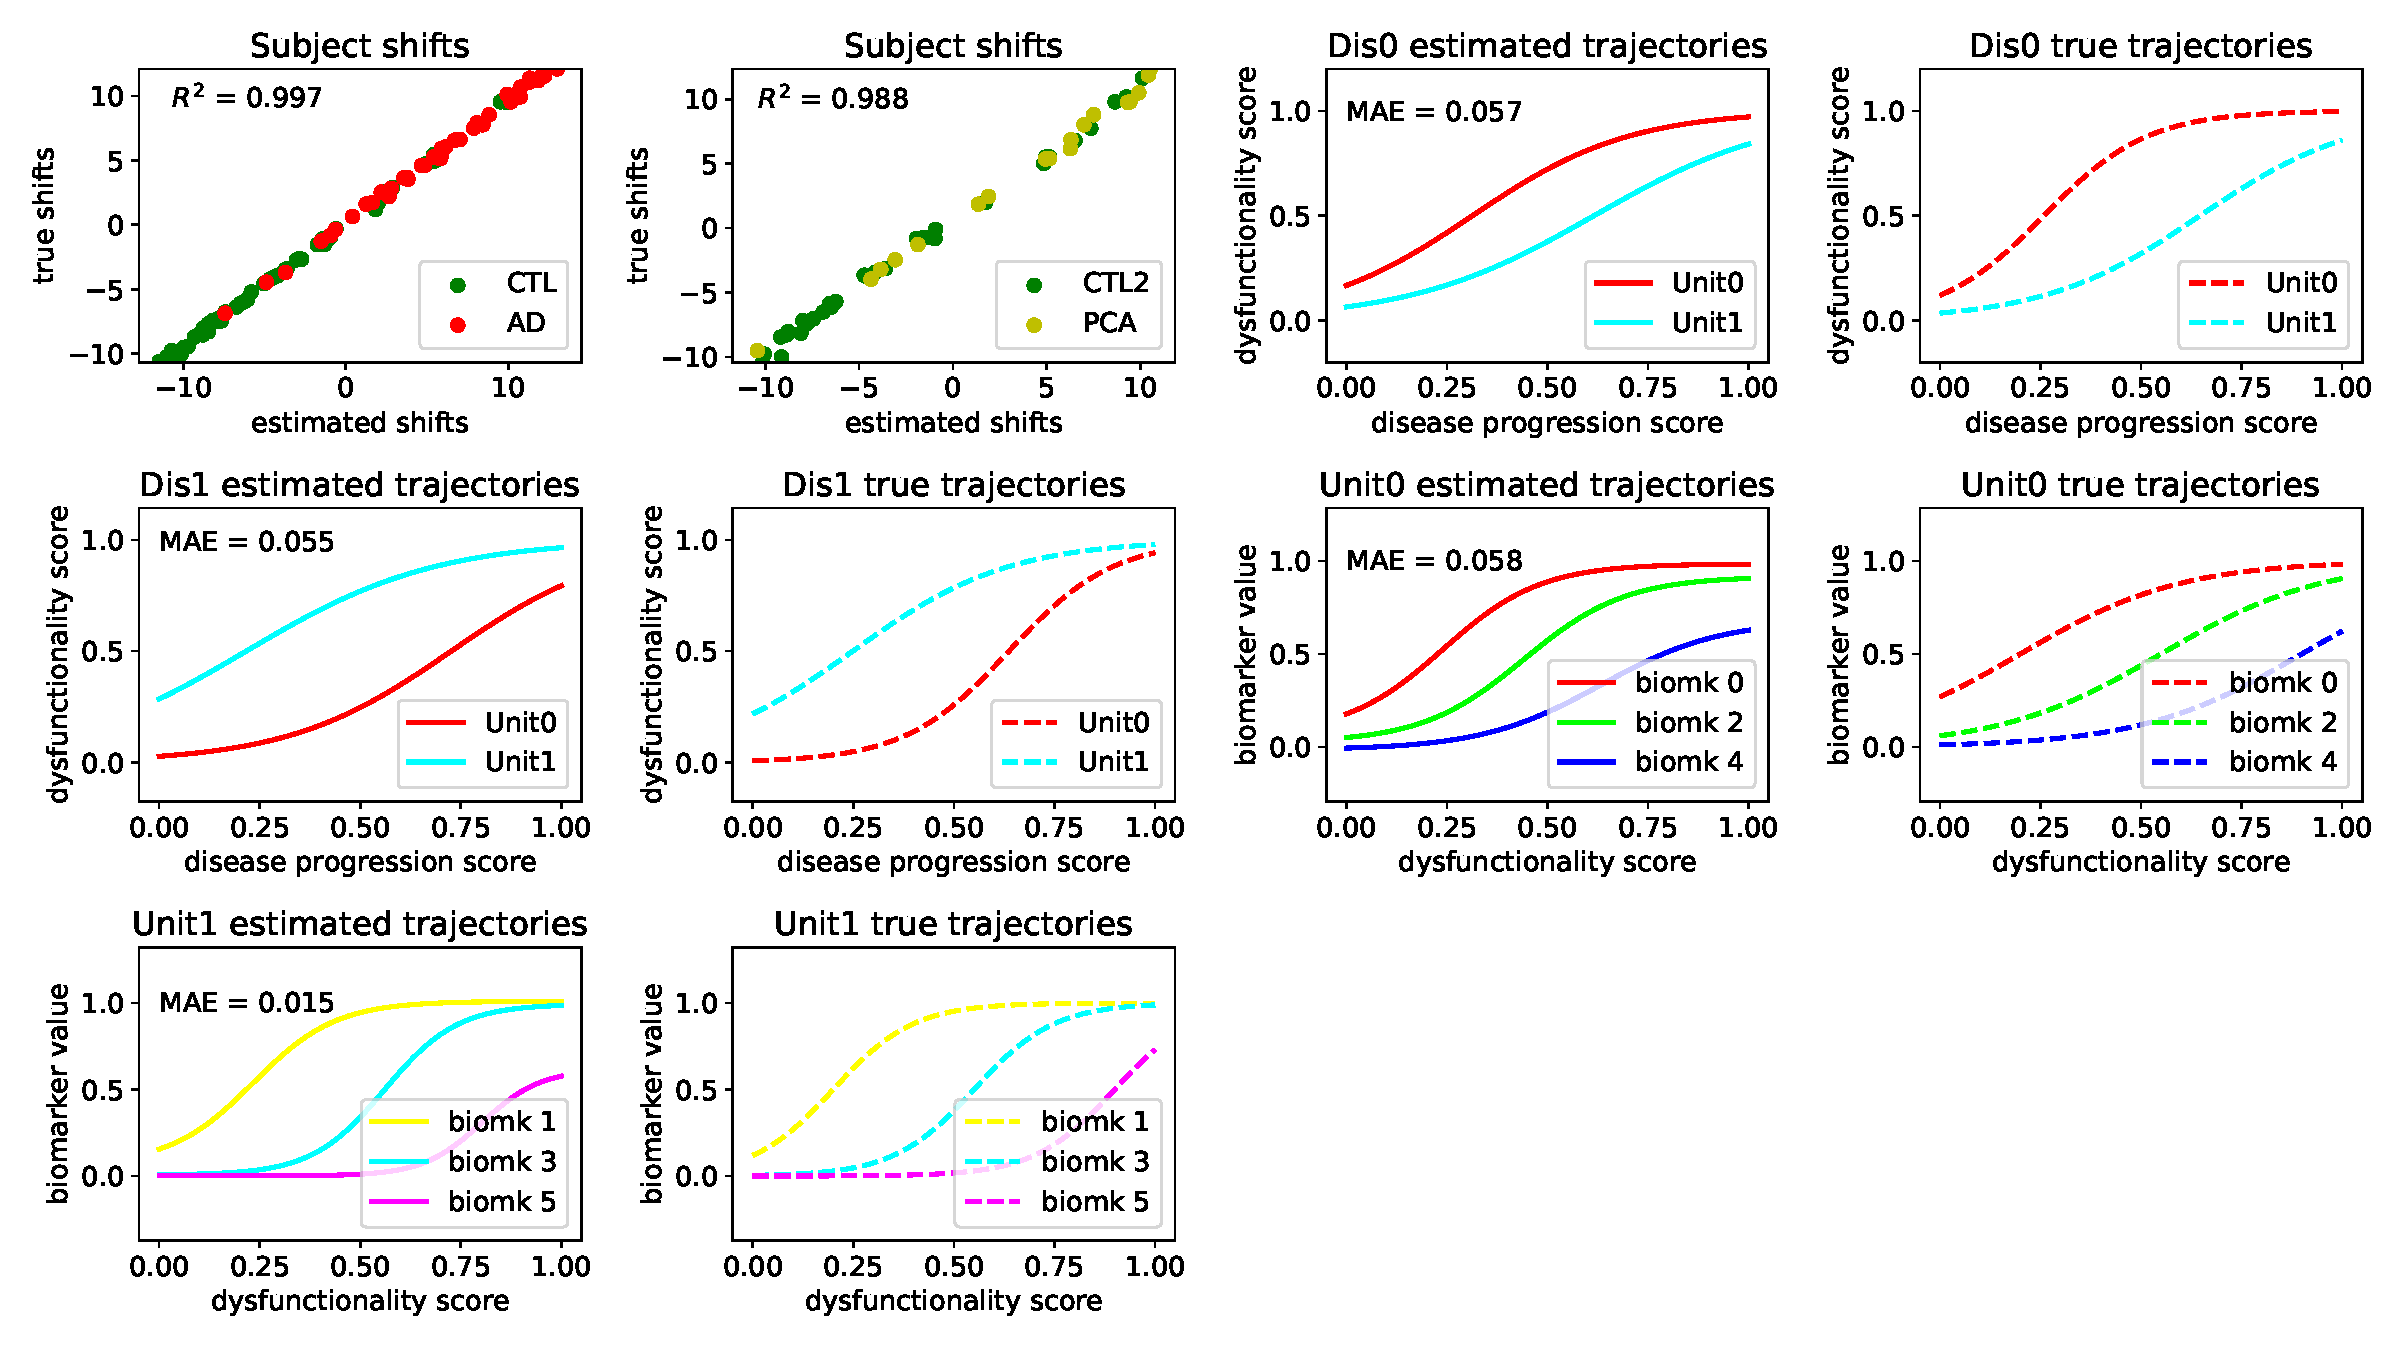
\includegraphics[width=\textwidth]{\jmdFld/resfiles/synth/synth1_JMD/compTrueParams101_synth1_JMD.pdf}
 \caption[DKT Simulation Results - Comparison between true and DKT-estimated biomarker trajectories and subject time-shifts.]{Comparison between true and DKT-estimated subject time-shifts and biomarker trajectories. (top-left) Scatter plots of the true shifts (y-axis) against estimated shifts (x-axis), for the 'synthetic AD' (left) and 'synthetic PCA' (right) diseases. We also show the DKT-estimated and true trajectories of the agnostic units within the 'synthetic AD' disease (top-right) and the 'synthetic PCA' disease (middle-left). For these figures, the x-axis measures the normalised disease progression score $s_i$ while the y-axis measures the dysfunctionality scores $f(s_i;\lambda_d^l)$. Finally, we also show the biomarker trajectories within unit 0 (middle-right) and unit 1 (bottom), where the x-axis represents the dysfunctionality scores $f(s_i;\lambda_d^l)$ and the y-axis represents the biomarker value.}
 \label{fig:dktSynthTrajCompTrue}
\end{figure}

\begin{figure}
\includegraphics[width=\textwidth]{\jmdFld/resfiles/synth/synth1_JMD/trajDisSpaceDis1_101_synth1_JMD.pdf}
 \caption[Estimated biomarker trajectories for the "synthetic PCA" disease, plotted alongside true trajectories]{Estimated biomarker trajectories for the "synthetic PCA" disease, plotted alongside true trajectories. Estimation of the trajectories in biomarkers 0,1,4 and 5 has been done without any data from the "synthetic PCA" disease, only based on the disease-agnostic correlations with biomarkers 2 and 3.}
 \label{fig:dktSynthTrajDrcSpace}
\end{figure}



\subsection{Results on TADPOLE and DRC Datasets}
\label{sec:dktResTadDrc}

% Fig1: biomarker traj. over dysfunction scores in one agnostic unit -> Fig2: dysfunction trajectories over disease stage in the two disease models -> Fig3: inferred biomarker trajectories "directly" over disease stage  in PCA
Fig. \ref{fig:pcaTadDisSpace} shows the estimated biomarker trajectories within the \emph{occipital unit} plotted over the dysfunction scores, along with samples from the model posterior and aligned subject data. The X-axis shows the dysfunctionality scores within the occipital unit, which represent estimated time-shifts, in months, from an arbitrary reference X=0, while the Y-axis shows biomarker values normalised to [0,1] range. The model shows an unbiased data fit (Fig. \ref{fig:pcaTadDisSpace}A), and we can observe most PCA subjects having abnormal occipital volumes, thus leading to high occipital dysfunctionality scores, in line with the current understanding of PCA as affecting posterior regions \cite{crutch2012posterior}. We also show the progression of dysfunctionality scores over the disease stage for typical AD (Fig \ref{fig:pcaTadDisSpace}B) and PCA (Fig \ref{fig:pcaTadDisSpace}C). In typical AD, we see that hippocampal dysfunction becomes abnormal earliest, while PCA shows early hippocampal dysfunction, which is later exceeded by the dysfunction in the occipital, temporal and parietal regions, which are known to be affected in PCA \cite{crutch2012posterior,Baron2001}. 

In Fig. \ref{fig:PCAtrajByModality}, we plot the inferred biomarker trajectories for PCA directly across the disease progression. We do this for five different modalities: MRI Volumes, DTI, FDG, AV45 and AV1451. The results again recapitulate known patterns in PCA, where posterior regions are predominantly affected in all modalities. However, for MRI volumes and AV45, we also see early abnormalities, which we attribute to the models underestimating the biomarker measurement noise.



% PCA vs tAD disease space
% \vspace{-2em}
\begin{picture}(5,5)
\put(0,-70){\textbf{\Large{A}}}
\end{picture}
\begin{figure}[H]
\centering
\begin{subfigure}{\textwidth}
\centering
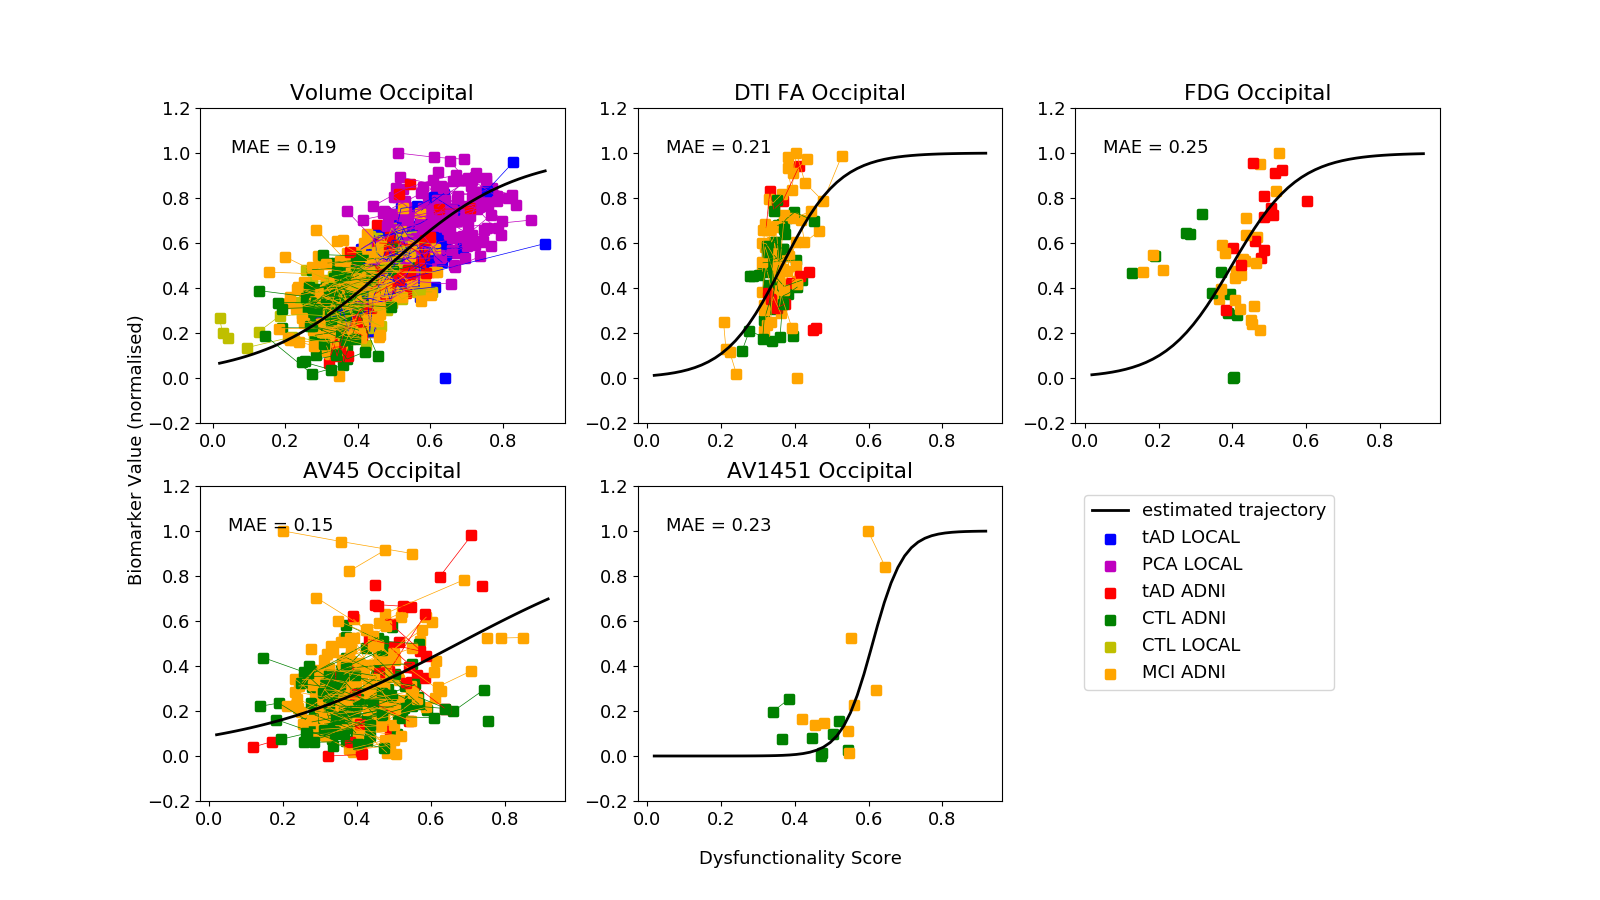
\includegraphics[width=0.8\textwidth, trim=90 0 110 0, clip]{\expFld/unit1_allTraj.png} 
% \caption{}
% \label{fig:occipUnit}
\end{subfigure}

\begin{picture}(5,5)
\put(0,20){\textbf{\Large{B}}}
\end{picture}
\begin{subfigure}{0.47\textwidth}
\centering
% typical AD\\
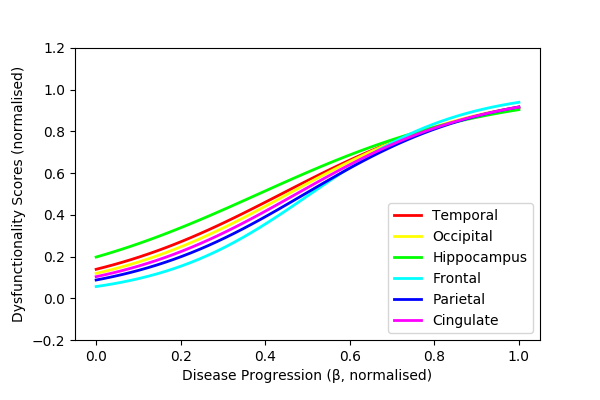
\includegraphics[width=0.8\textwidth, trim=0 0 0 20, clip]{\expFld/dis0_tAD_allTrajZeroOne.png} 
% \caption{C}
\end{subfigure}
\begin{picture}(5,5)
\put(0,20){\textbf{\Large{C}}}
\end{picture}
\begin{subfigure}{0.47\textwidth}
\centering
% PCA\\
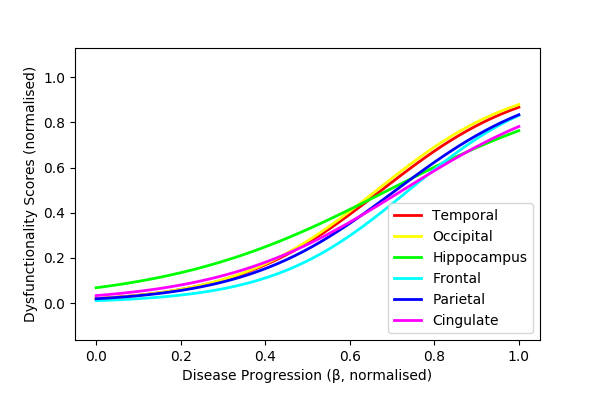
\includegraphics[width=0.8\textwidth, trim=0 0 0 20, clip]{\expFld/dis1_PCA_allTrajZeroOne.png} 
% \caption{PCA}
\end{subfigure}
\caption{(A) Estimated biomarker trajectories in the occipital agnostic unit. Subject data from ADNI and our local cohort are also shown. The X-axis, defined as the occipital dysfunctionality score, represents the time-shifts (in months) of each subject. Red lines represent samples from the trajectory posterior. The Y-axis measures biomarker values (normalised). (B-C) Progression of dysfunctionality scores for (B) typical AD and (C) PCA.}
\label{fig:pcaTadDisSpace}
\end{figure}



% estimated (hypothetical) trajectories in PCA: DTI, FDG, AV45, AV1451.Volumetric trajectories were based on PCA MRI data.
\begin{figure}
 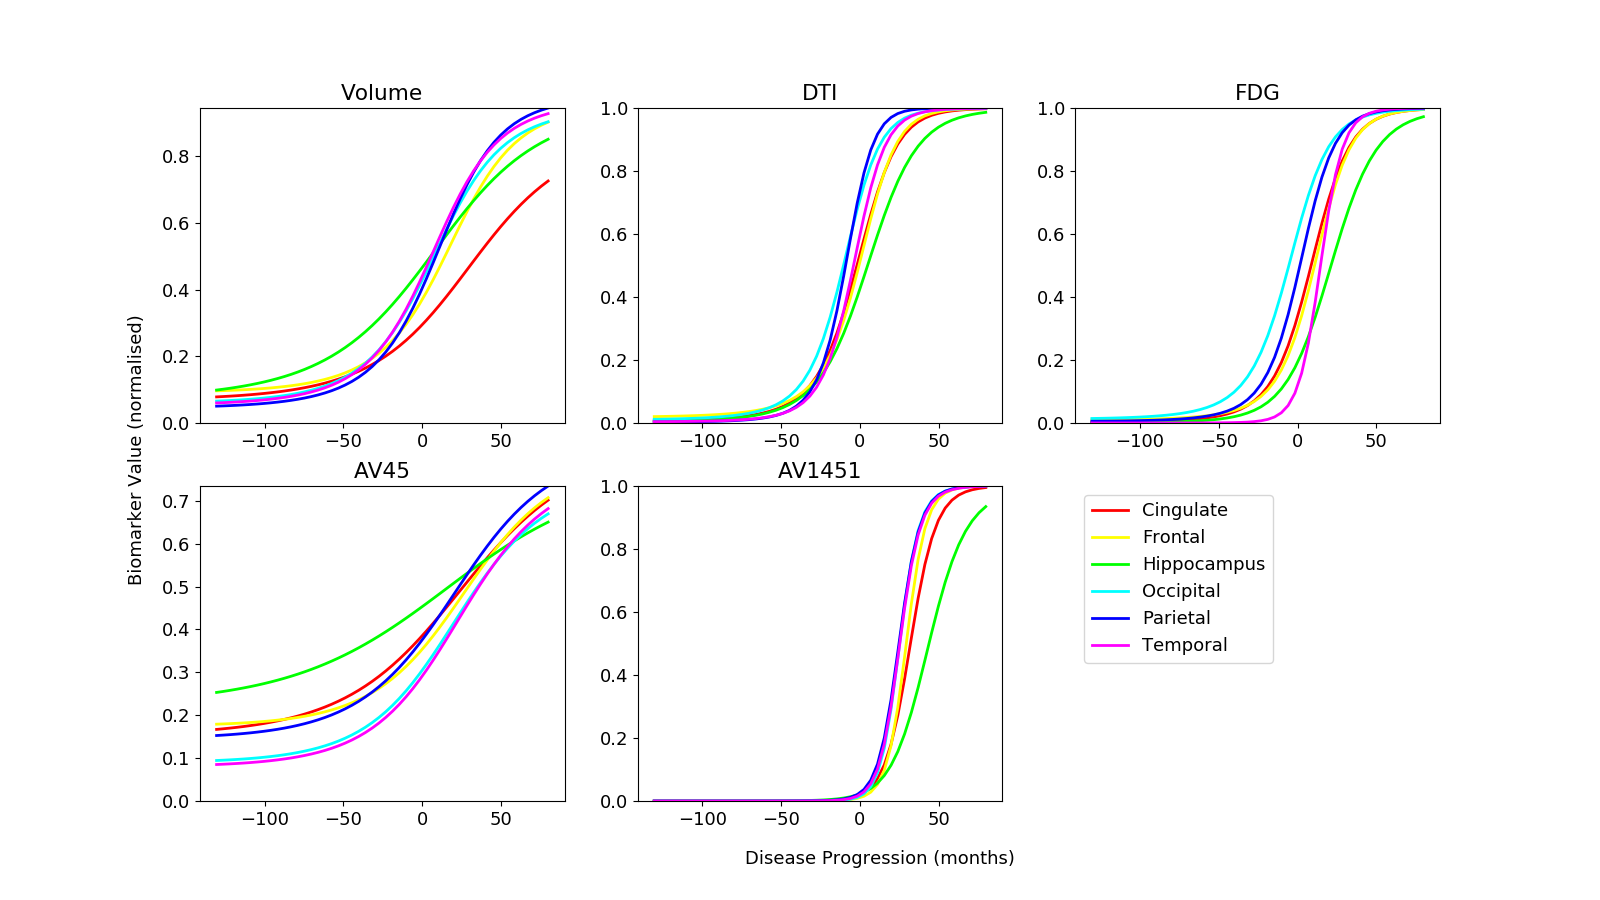
\includegraphics[width=\textwidth, trim=0 20 0 0, clip]{\expFld/trajDisSpaceOverlap_PCA_tad-drcTinyPen5_JMD.png}
 \caption{Estimated trajectories for the PCA cohort. The only data that were available were the MRI volumetric data. The dynamics of the other biomarkers has been inferred by the model using data from typical AD, and taking into account the different spatial distribution of pathology in PCA as compared to typical AD.}
 \label{fig:PCAtrajByModality}
\end{figure}


\section{Validation on DTI Data in PCA}
\label{sec:dktResVal}

We validated our model using a separate test set of 20 DTI scans from controls and PCA patients from the DRC cohort. We used DKT to predict the DTI biomarker values for the subjects within the unseen test set, using only their MRI biomarkers. Table \ref{sec:dktPerfMetrics} shows the prediction mean squared error (MSE) and rank correlation between the DKT-predicted biomarker values and the measured values. We computed the rank correlation in order to remove the effect of any systemic biases due to the completely different progressive disease and dataset that we are predicting on. We also show similar performance metrics for two simpler models:
\begin{itemize}
 \item Latent stage model: a sigmoidal based disease progression model, as described in \cite{jedynak2012computational}. This model assumes all tAD and PCA subjects follow the same progression.
 \item Linear model: a linear univariate regression model that predicts the DTI biomarker based on the corresponding MRI biomarker, independently for each region.
\end{itemize}

The results from Table \ref{sec:dktPerfMetrics} indicate that the DKT predictions are relatively small for the frontal, occipital, temporal and parietal areas. Moreover, rank correlation of the DKT predicted values is also high for the cingulate lobe and the hippocampus. In terms of model comparison, DKT has better performance than the linear model (all results significant with $p < 0.002$, Bonferroni corrected), since it uses information across all brain regions instead of assuming independence across regions. While DKT has similar performance to the latent stage model, it does not assume that the diseases have the same progression and it allows us to understand mechanisms that are shared between related diseases. 

\newcommand{\cw}{c}

\begin{table}
\footnotesize
\begin{tabular}{c | c c c c c c}
\textbf{Model} & \textbf{Cingulate} & \textbf{Frontal} & \textbf{Hippo.} & \textbf{Occip.} & \textbf{Parietal} & \textbf{Temporal}\\
& \multicolumn{6}{c}{\textbf{Prediction Error (MSE)}}\\
DKT & 0.09$\pm$0.04 & 0.03$\pm$0.01 & 0.18$\pm$0.03 & 0.04$\pm$0.02 & 0.06$\pm$0.02 & 0.04$\pm$0.02\\
Latent stage model & 0.09$\pm$0.04 & 0.03$\pm$0.01 & 0.17$\pm$0.03 & 0.04$\pm$0.02 & 0.06$\pm$0.02 & 0.04$\pm$0.02\\
Linear Model & 0.05$\pm$0.02* & 0.15$\pm$0.04* & 0.09$\pm$0.03* & 0.07$\pm$0.03* & 0.07$\pm$0.02* & 0.07$\pm$0.02*\\
& \multicolumn{6}{c}{\textbf{Rank Correlation (Spearman rho)}}\\
DKT  & 0.76  & 0.48  & 0.76  & 0.55  & 0.55  & 0.33 \\
Latent stage model  & 0.76  & 0.49  & 0.80*  & 0.56  & 0.51*  & 0.33 \\
Linear Model  & 0.48*  & 0.31*  & 0.64*  & 0.61*  & 0.57*  & 0.27* \\
\end{tabular}
\normalfont
\caption[Performance evaluation of DKT and two simpler models]{Performance evaluation of DKT and two simpler models: a latent stage disease progression model and a linear univariate model of DTI predicted from MRI. The top table shows the prediction error (MSE) while the bottom table shows the rank correlation measured by Spearman's rho. (*) Statistically significant difference between the current model performance and DKT, based on a two-tailed t-test, Bonferroni corrected.}
\label{sec:dktPerfMetrics}
\end{table}

\section{Discussion}
\label{sec:dktDis}

We presented DKT, a framework that enables, for the first time, joint modelling of biomarker progressions in multiple neurodegenerative diseases simultaneously. The framework allows the inference of biomarker trajectories in rare diseases, for which there is not enough data to allow estimation of such trajectories, and accounts for a different spatial distribution of pathology between distinct phenotypes. This further enables us to understand the complex mechanisms of rare diseases, as well as mechanisms shared between different types of related diseases.

We provided an example implementation of DKT using specific models of the biomarker trajectories, measurement noise and link function (the disease progression score). However, DKT should be considered as a general framework for joint modelling of biomarker trajectories within different diseases simultaneously. The actual implementation of DKT can thus be extended to use non-parametric trajectories, or more complex link functions that estimate not only subject time-shifts but also progression speed or higher order terms.

While in this work we have focused on Alzheimer's variants such as tAD and PCA, DKT can also be applied to other progressive neurodegenerative diseases of non-Alzheimer's type such as tauopathies (e.g. Frontotemporal dementia), synucleinopathies (e.g. Parkinson's disease), other neurodegenerative diseases such as Huntington's disease or Multiple Sclerosis, and even the normal ageing process. Cognitive tests can also be included in the disease-specific sub-models of DKT, or even allocated in the agnostic units of the regions that are responsible for those tasks, based on previous voxel-based morphometry studies. However, some care needs to be exercised when selecting the biomarkers and grouping them into agnostic units, as in some diseases the assumption of disease agnostic dynamics might not hold for some groups of molecular biomarkers. For example, some non-Alzheimer's tauopathies such as Frontotemporal dementia might show tau abnormalities but no corresponding amyloid abnormalities within the same region. In the case of Frontotemporal dementia, we recommend including higher-level biomarkers such as glucose metabolism from FDG, white matter degeneration from DTI or volume from structural MRI, but one should exclude amyloid markers. 

Our work has several limitations: 1) DKT assumes all subjects within a disease follow the same trajectory, without considering heterogeneity within the disease population, 2) the allocation of biomarkers into agnostic units has to be done using \emph{a-priori} human knowledge, 3) DKT currently works only on extracted brain features, discarding important information present in the brain morphometry, 4) for validation, the synthetic experiment we ran was limited to only one setting of the parameters and 5) the validation on patient data was also done only on a small set of 20 DTI scans, due to lack of multimodal data in PCA.

There are several potential avenues for further research: 1) to account for heterogeneity, DKT can also be easily extended to include subject-specific effects; 2) improved schemes for biomarker allocation to agnostic units can take connectivity into account, or derive it from the data automatically; 3) to account for brain morphometry and connectivity, DKT can be extended into a fully spatio-temporal model, by estimating continuous changes in volumetric brain images -- in this case, each voxel can have an associated dysfunctionality score that is derived from measurements of various modalities from that voxel; 4-5) DKT can be further validated on more complex synthetic experiments with variable parameter settings, and on patient data from ADNI, where the population could be \emph{a-priori} split into sub-groups with different progressions. On these subgroups, DKT can be used to transfer biomarker modalities that have been left out during training.

%
% ---- Bibliography ---- 
% USE HARVARD STANDARD

\bibliographystyle{unsrtnat}
\begin{thebibliography}{5}

\bibitem{lorenzi2017disease}
Lorenzi, M., Filippone, M., Alexander, D.C. and Ourselin, S., 2017. Disease Progression Modeling and Prediction through Random Effect Gaussian Processes and Time Transformation. arXiv preprint arXiv:1701.01668.


\bibitem{oxtoby2018}
Oxtoby, N.P., Young, A.L., Cash, D.M., Benzinger, T.L., Fagan, A.M., Morris, J.C., Bateman, R.J., Fox, N.C., Schott, J.M. and Alexander, D.C., 2018. Data-driven models of dominantly-inherited Alzheimer's disease progression. bioRxiv, p.250654.


\bibitem{iturria2016early}
Iturria-Medina, Y., Sotero, R.C., Toussaint, P.J., Mateos-Pérez, J.M., Evans, A.C., Weiner, M.W., Aisen, P., Petersen, R., Jack, C.R., Jagust, W. and Trojanowki, J.Q., 2016. Early role of vascular dysregulation on late-onset Alzheimer's disease based on multifactorial data-driven analysis. Nature communications, 7, p.11934.


\bibitem{young2014data}
Young, A.L., Oxtoby, N.P., Daga, P., Cash, D.M., Fox, N.C., Ourselin, S., Schott, J.M. and Alexander, D.C., 2014. A data-driven model of biomarker changes in sporadic Alzheimer's disease. Brain, 137(9), pp.2564-2577.


\bibitem{young2018uncovering}
Young, A.L., Marinescu, R.V., Oxtoby, N.P., Bocchetta, M., Yong, K., Firth, N.C., Cash, D.M., Thomas, D.L., Dick, K.M., Cardoso, J. and van Swieten, J., 2018. Uncovering the heterogeneity and temporal complexity of neurodegenerative diseases with Subtype and Stage Inference. Nature communications, 9(1), p.4273.

\bibitem{scelsi2018genetic}
Scelsi, M.A., Khan, R.R., Lorenzi, M., Christopher, L., Greicius, M.D., Schott, J.M., Ourselin, S. and Altmann, A., 2018. Genetic study of multimodal imaging Alzheimer's disease progression score implicates novel loci. Brain.


\bibitem{hon2017towards}
Hon, M. and Khan, N., 2017. Towards Alzheimer's Disease Classification through Transfer Learning. arXiv preprint arXiv:1711.11117.


\bibitem{cheng2017multi}
Cheng, B., Liu, M., Shen, D., Li, Z., Zhang, D. and Alzheimer's Disease Neuroimaging Initiative, 2017. Multi-domain transfer learning for early diagnosis of Alzheimer's disease. Neuroinformatics, 15(2), pp.115-132.

\bibitem{cheng2015domain}
Cheng, B., Liu, M., Zhang, D., Munsell, B.C. and Shen, D., 2015. Domain transfer learning for MCI conversion prediction. IEEE Transactions on Biomedical Engineering, 62(7), pp.1805-1817.

\bibitem{marinescu2018tadpole}
Marinescu, R.V., Oxtoby, N.P., Young, A.L., Bron, E.E., Toga, A.W., Weiner, M.W., Barkhof, F., Fox, N.C., Klein, S. and Alexander, D.C., 2018. TADPOLE Challenge: Prediction of Longitudinal Evolution in Alzheimer's Disease. arXiv preprint arXiv:1805.03909.


\bibitem{sabuncu2011dynamics}
Sabuncu, M.R., Desikan, R.S., Sepulcre, J., Yeo, B.T.T., Liu, H., Schmansky, N.J., Reuter, M., Weiner, M.W., Buckner, R.L., Sperling, R.A. and Fischl, B., 2011. The dynamics of cortical and hippocampal atrophy in Alzheimer disease. Archives of neurology, 68(8), pp.1040-1048.

\bibitem{jedynak2012computational}
Jedynak, B.M., Lang, A., Liu, B., Katz, E., Zhang, Y., Wyman, B.T., Raunig, D., Jedynak, C.P., Caffo, B., Prince, J.L. and Alzheimer's Disease Neuroimaging Initiative, 2012. A computational neurodegenerative disease progression score: method and results with the Alzheimer's disease Neuroimaging Initiative cohort. Neuroimage, 63(3), pp.1478-1486.

\bibitem{Ossenkoppele2014atrophy}
Ossenkoppele, R., Cohn‐Sheehy, B.I., La Joie, R., Vogel, J.W., Möller, C., Lehmann, M., van Berckel, B.N., Seeley, W.W., Pijnenburg, Y.A., Gorno‐Tempini, M.L. and Kramer, J.H., 2015. Atrophy patterns in early clinical stages across distinct phenotypes of Alzheimer's disease. Human brain mapping, 36(11), pp.4421-4437.

\bibitem{crutch2012posterior}
Crutch, S.J., Lehmann, M., Schott, J.M., Rabinovici, G.D., Rossor, M.N. and Fox, N.C., 2012. Posterior cortical atrophy. The Lancet Neurology, 11(2), pp.170-178.


\bibitem{Baron2001}
Baron, J.C., Ch\'{e}telat, G., Desgranges, B., Perchey, G., Landeau, B., {de la Sayette}, V. and Eustache, F., 2001. NeuroImage 14(2), pp.298-309.



\end{thebibliography}

\clearpage

\end{document}

